\chapter{\label{chp:toolflowex}Tool-flow example}
To give you a general idea of how the tool-flow works, this section will give a simple example starting with the C-code and show the output all the way through HLS, simulation, synthesis, layout and power analysis. \Cref{lst:ccodelisting} shows a simple C-program with two functions, \textit{main} and \textit{squared}. The \textit{main}-function will be the top function and this function takes three input parameters, \textit{done}, \textit{inData} and \textit{\_\_out\_outData}. The \textit{main}-function contains a while loop, which will run as long as the input parameter \textit{done} is set to zero. Inside the loop the function \textit{squared} is called with the argument from \textit{inData} and the return value from \textit{squared} is assigned to the input argument \textit{\_\_out\_outData}. If you are familiar with C programming, you might think that it is a weird thing to be assigning values to the inputs, but as described in \cref{sec:assValueToOutput}, this is implemented as a way to get multiple outputs to the generated module. Notice also the \textit{volatile} keyword in the declaration of the \textit{\_\_out\_outData} parameter, as this is a necessary part of the generating outputs.
\lstset{language=C++,style=Cstyle}
\begin{lstlisting}[caption={Simple C-code example},label=lst:ccodelisting]
int squared (int base) {
  return base * base;
}

int main (int done, int inData, volatile int __out_outData) {
  while(done == 0) {
    __out_outData = squared(inData);
  }
  return 0;
}
\end{lstlisting}

\section{HLS with LegUp}
The HLS-tool is the only part of the tool-flow located on another computer than the rest. This is not an issue when running a single design through the tool-flow, as the file can simply be copy-pasted to the destination. As described in \
\subsection{Constraint files}
LegUp uses constraint files to set constraints and settings for the \gls{hls}. The default values for necessary constraints is set in the default constraint-file located in \textasciitilde/legup4-0/example/legup.tcl. The default constraints can be overridden by adding a local constraint file. The filename of the local constraint file need to be specified in the Makefile for the constraints to take effect. This is done by adding the line \verb!LOCAL_CONFIG = -legup-config=config.tcl! to the Makefile, where config.tcl is the filename of the local constraint-file. 
\subsection{Makefile}
The minimal local Makefile of LegUp contains the following three lines:
\begin{verbatim}
  NAME=name
  LEVEL = ..
  include $(LEVEL)/Makefile.common
\end{verbatim}

The Variable \textit{NAME} is the name of the design. This variable will be used to name the output-files of the design. The Variable \textit{LEVEL} indicated the number of directory levels it is up to where the common Makefile is located. 1 level up is marked as .., 2 levels up is marked as ../.. and so on, just like in a standard Linux shell. Other parameters, like \textit{NO\_OPT} (disable optimization in the compilator) and \textit{NO\_INLINE} (avoid inlining functions in the program), can also be added to the Makefile for passing flags and settings to the compilation. In some cases, especially with simple test-programs, these two flags are necessary to prevent the compiler from optimize away the whole program.

The C-code is compilated into LLVM \gls{ir} using the clang frontend for the LLVM compilation framework. The initial result before any \gls{lto} is performed is shown in \cref{lst:llvmirprelto}. If you are familiar with assembly code, you might understand some of the operations, like alloca, load, store, mul and icmp. Each define block corresponds to one function from the C-code. The main function, which contains a while-loop, is split into multiple labels. The first section refers to the input parameters and memory allocation and storing of these. Temporary registers, declared on the form \%1, \%2 .. \%N, are inserted where needed. The section from the line "\textit{; <label>:4}" is the checking of the condition of the while loop. Further, \textit{label 7} is operations inside the while loop, and \textit{label 10} is operations after the loop has exited.
\lstset{language=llvm,style=LLVMstyle}
\begin{lstlisting}[caption={LLVM IR before LTO},label=lst:llvmirprelto]
define i32 @squared(i32 %base) #0 {
  %1 = alloca i32, align 4
  store i32 %base, i32* %1, align 4
  %2 = load i32* %1, align 4
  %3 = load i32* %1, align 4
  %4 = mul nsw i32 %2, %3
  ret i32 %4
}

; Function Attrs: noinline nounwind
define i32 @main(i32 %done, i32 %inData, i32 %__out_outData) #0 {
  %1 = alloca i32, align 4
  %2 = alloca i32, align 4
  %3 = alloca i32, align 4
  store i32 %done, i32* %1, align 4
  store i32 %inData, i32* %2, align 4
  store volatile i32 %__out_outData, i32* %3, align 4
  br label %4

; <label>:4                              ; preds = %7, %0
  %5 = load i32* %1, align 4
  %6 = icmp eq i32 %5, 0
  br i1 %6, label %7, label %10

; <label>:7                              ; preds = %4
  %8 = load i32* %2, align 4
  %9 = call i32 @squared(i32 %8) #1
  store volatile i32 %9, i32* %3, align 4
  br label %4

; <label>:10                             ; preds = %4
  ret i32 0
}
\end{lstlisting}
By default, some optimization passes are run on the \gls{ir} to remove unnecessary operations and reduce the number of registers needed. All available passes are described in \cite{llvmpasses}, but the ones that is run by default is \textit{mem2reg}, \textit{instcombine}, \textit{loops}, \textit{loop-simplify}, \textit{basicaa}, \textit{indvars}, \textit{loop-pipeline}, \textit{internalize}, and \textit{globaldce}. These passes analyses, simplifies and removes operations. The result is listed in \cref{lst:llvmirpostlto}. Notice that the only stores left in the code is the ones connected to the input parameter declared as volatile. The keyword volatile, which definition is \textit{likely to change suddenly and unexpectedly}, tells the compiler to avoid performing optimizations on this object, as it might change in an unexpected way. This is what we want, as assigning values to an input parameter in C does not make sense, and would therefore have been optimized away. 

\begin{lstlisting}[caption={LLVM IR after LTO},label=lst:llvmirpostlto]
define internal i32 @squared(i32 %base) #0 {
  %1 = mul nsw i32 %base, %base
  ret i32 %1
}

; Function Attrs: noinline nounwind
define i32 @main(i32 %done, i32 %inData, i32 %__out_outData) #0 {
  %1 = alloca i32, align 4
  store volatile i32 %__out_outData, i32* %1, align 4
  br label %2

; <label>:2                              ; preds = %4, %0
  %3 = icmp eq i32 %done, 0
  br i1 %3, label %4, label %6

; <label>:4                              ; preds = %2
  %5 = call i32 @squared(i32 %inData) #1
  store volatile i32 %5, i32* %1, align 4
  br label %2

; <label>:6                              ; preds = %2
  ret i32 0
}
\end{lstlisting}

Also notice that the storing and loading of the other input parameters has been swapped by referencing the input parameter register directly. For instance the four lines:

\begin{lstlisting}
%2 = alloca i32, align 4
store i32 %inData, i32* %2, align 4
%8 = load i32* %2, align 4
%9 = call i32 @squared(i32 %8) #1
\end{lstlisting}
has been transformed into the single line:
\begin{lstlisting}
%5 = call i32 @squared(i32 %inData) #1
\end{lstlisting}
The LegUp backend pass for LLVM is run on the \gls{ir} to generate Verilog-output. LegUp perfomes allocation, scheduling and builds RTL models of the functionality, based on given constraints. These RTL models are printed to a file as Verilog HDL. \cref{lst:verilogmodule1} shows the declaration of the \textit{main}-module, parameters representing states, port and internal signal declarations and instantiation of sub-modules.
\lstset{language=Verilog, style=VerilogStyle}
\begin{lstlisting}[caption={Verilog module, port, signal and parameter declaration, and sub-module instantiation},label=lst:verilogmodule1]
module main
(
	clk,
	clk2x,
	clk1x_follower,
	reset,
	start,
	finish,
	memory_controller_waitrequest,
	return_val,
	arg_done,
	arg_inData,
	arg_outData,
	arg_outData_valid,
	iterationFinish
);

parameter [3:0] LEGUP_0 = 4'd0;
parameter [3:0] LEGUP_F_main_BB__0_1 = 4'd1;
parameter [3:0] LEGUP_F_main_BB__0_2 = 4'd2;
parameter [3:0] LEGUP_F_main_BB__2_3 = 4'd3;
parameter [3:0] LEGUP_F_main_BB__4_4 = 4'd4;
parameter [3:0] LEGUP_F_main_BB__4_6 = 4'd6;
parameter [3:0] LEGUP_F_main_BB__4_7 = 4'd7;
parameter [3:0] LEGUP_F_main_BB__6_8 = 4'd8;
parameter [3:0] LEGUP_function_call_5 = 4'd5;

input  clk;
input  reset;
input  start;
output reg  finish;
input  memory_controller_waitrequest;
output reg [31:0] return_val;
input [31:0] arg_done;
input [31:0] arg_inData;
output reg [31:0] arg_outData;
output reg  arg_outData_valid;
output reg  iterationFinish;
reg [3:0] cur_state;
reg [3:0] next_state;

squared squared (
	.memory_controller_waitrequest (memory_controller_waitrequest),
	.clk (clk),
	.clk2x (clk2x),
	.clk1x_follower (clk1x_follower),
	.reset (reset),
	.start (squared_start),
	.finish (squared_finish),
	.return_val (squared_return_val),
	.arg_base (squared_arg_base)
);
\end{lstlisting}
LegUp generates an FSM that performs calculations and generates output. The generated FSM controller for the above example code is listed in \cref{lst:verilogfsm}, and the state diagram of the FSM is shown in \cref{fig:verilogfsm}.
\begin{lstlisting}[caption={Verilog FSM},label=lst:verilogfsm]
always @(posedge clk) begin
if (reset == 1'b1)
	cur_state <= LEGUP_0;
else if (memory_controller_waitrequest == 1'd1)
	cur_state <= cur_state;
else
	cur_state <= next_state;
end

always @(*)
begin
next_state = cur_state;
case(cur_state)  // synthesis parallel_case  
LEGUP_0:
	if ((start == 1'd1))
		next_state = LEGUP_F_main_BB__0_1;
LEGUP_F_main_BB__0_1:
		next_state = LEGUP_F_main_BB__0_2;
LEGUP_F_main_BB__0_2:
		next_state = LEGUP_F_main_BB__2_3;
LEGUP_F_main_BB__2_3:
	if ((main_2_3 == 1'd1))
		next_state = LEGUP_F_main_BB__4_4;
	else if ((main_2_3 == 1'd0))
		next_state = LEGUP_F_main_BB__6_8;
LEGUP_F_main_BB__4_4:
		next_state = LEGUP_function_call_5;
LEGUP_F_main_BB__4_6:
		next_state = LEGUP_F_main_BB__4_7;
LEGUP_F_main_BB__4_7:
		next_state = LEGUP_F_main_BB__2_3;
LEGUP_F_main_BB__6_8:
		next_state = LEGUP_0;
LEGUP_function_call_5:
	if ((squared_finish_final == 1'd1))
		next_state = LEGUP_F_main_BB__4_6;
default:
	next_state = cur_state;
endcase
end
\end{lstlisting}
\begin{figure}[hbpt]
\centering
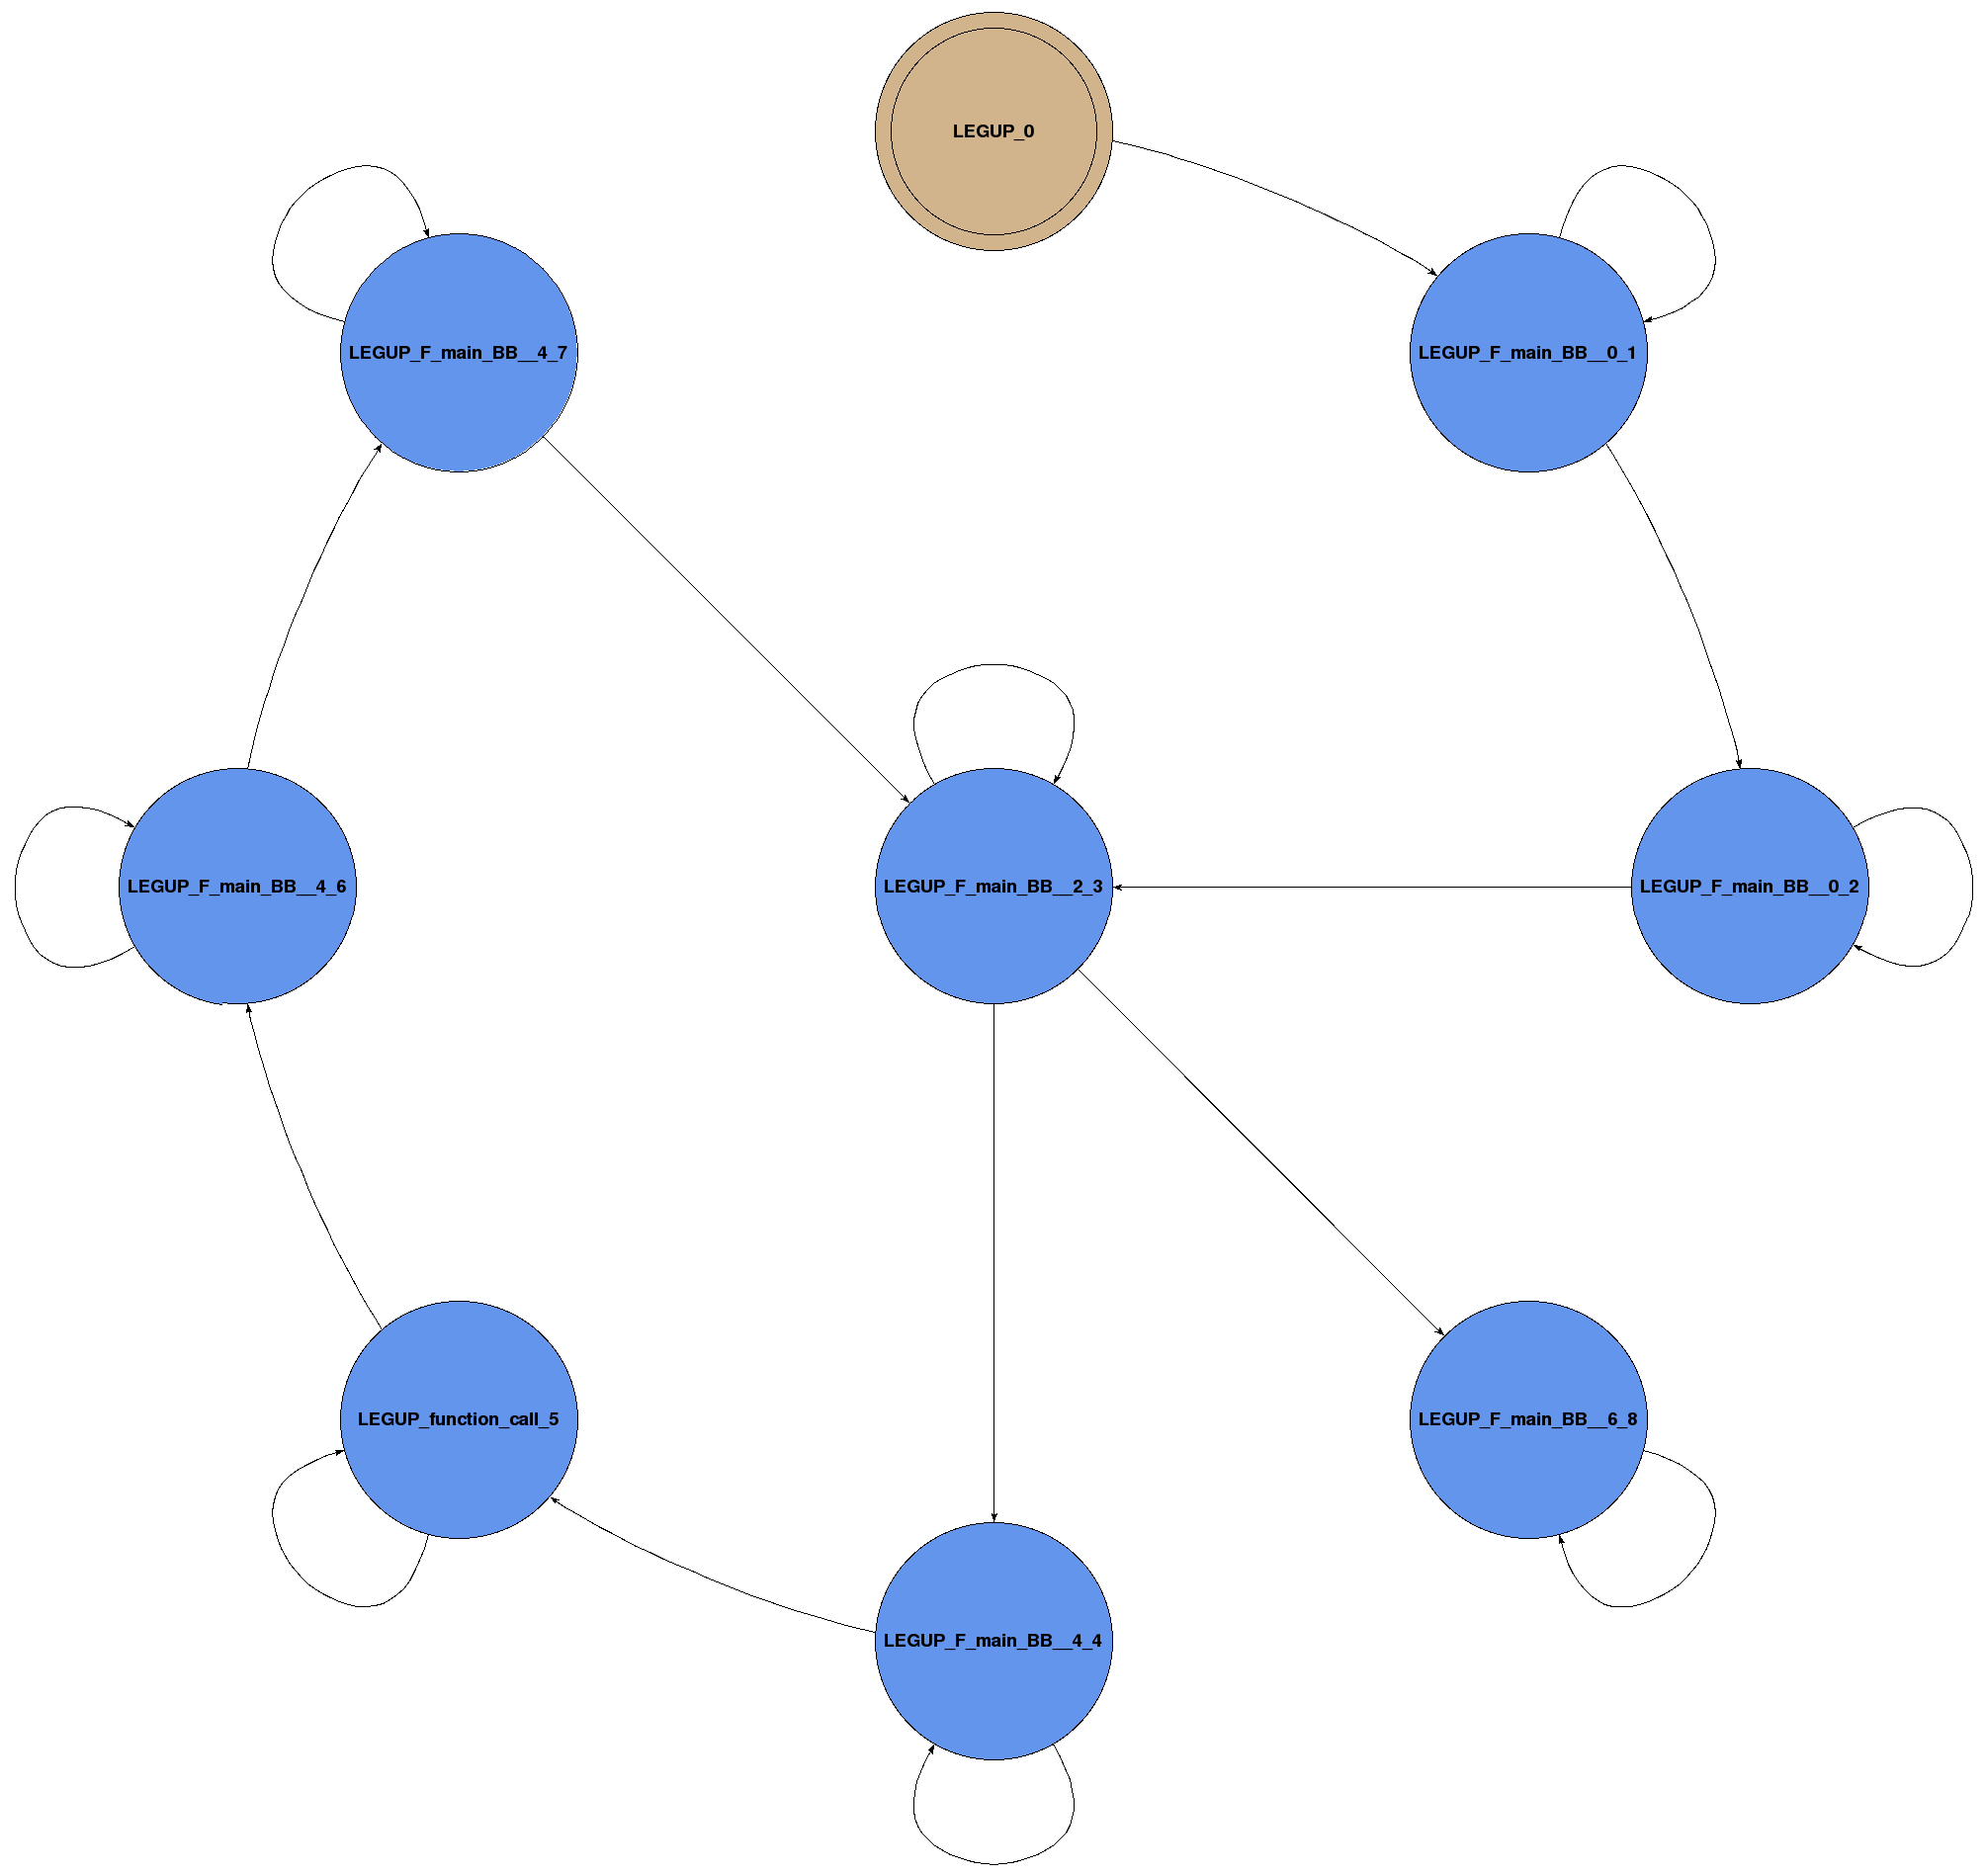
\includegraphics[width=0.99\textwidth]{../figs/VerilogFSM.png}
\caption{\label{fig:verilogfsm}State diagram of generated FSM}
\end{figure}
By looking at the state diagram, some parts from the C-code can be recognized. \textit{LEGUP\_0} is the initial state and the two following states is allocating and storing the volatile input parameter. \textit{LEGUP\_F\_main\_BB\_2\_3} is where the condition checking for the while loop is performed. The states below and left of the condition state is the states inside the while loop, and \textit{LEGUP\_F\_main\_BB\_6\_8} is the exit-state, signalizing the completion of the program.

Some signal assignments are shown in \cref{lst:verilogsignalassignment}. Each assignment is printed with the corresponding LLVM operation commented abowe, to increase readability of the code. The later assignment of output signals are not generated directly from an LLVM operation and does thus not have this operation printed along the assignment.
\begin{lstlisting}[caption={Verilog FSM},label=lst:verilogsignalassignment,float]
always @(*) begin
	/* main: %2*/
	/*   %3 = icmp eq i32 %done, 0*/
		main_2_3 = (arg_done == 32'd0);
end
always @(posedge clk) begin
	/* main: %4*/
	/*   %5 = call i32 @squared(i32 %inData) #1*/
	if ((cur_state == LEGUP_F_main_BB__4_4)) begin
		squared_arg_base <= arg_inData;
	end
end
always @(posedge clk) begin
	if ((cur_state == LEGUP_F_main_BB__4_6)) begin
		arg_outData <= main_4_5_reg;
	end
end
always @(posedge clk) begin
	if ((cur_state == LEGUP_F_main_BB__4_6)) begin
		arg_outData_valid <= 1'd1;
	end
	if (~((cur_state == LEGUP_F_main_BB__4_6))) begin
		arg_outData_valid <= 1'd0;
	end
end
always @(posedge clk) begin
	if ((cur_state == LEGUP_F_main_BB__4_7)) begin
		iterationFinish <= 1'd1;
	end
	if (~((cur_state == LEGUP_F_main_BB__4_7))) begin
		iterationFinish <= 1'd0;
	end
end
\end{lstlisting}

\section{Simulation}
\subsection{Simulation libraries}

LegUp generates local RAMs for each output-parameter to the main module, as these parameters needs to be declared as volatile. 

In the declaration of the modules ram\_dual\_port and rom\_dual\_port, a conversion function from an Altera library is used to convert .mif files to a format readable by Modelsim. The .mif-file contains initial content of memory. The code snippet that uses this library is shown in \cref{lst:alteralibrary}. If the design does not contain any initial memory values, this conversion method is not needed and could be removed from the design. As this is a feature in LegUp, this has not been altered at this time. This requires the library file to be included in the design filelist for simulation to be successful. The library-file is located in \textasciitilde/legup-4.0/ip/libs/altera/altera\_mf.v of the LegUp VirtualBox image. 
\lstset{language=Verilog, style=VerilogStyle}
\begin{lstlisting}[caption={Altera Library function used for memory management},label=lst:alteralibrary]
ALTERA_MF_MEMORY_INITIALIZATION mem ();
// modelsim can't read .mif files directly. So use Altera function to
// convert them to .ver files
mem.convert_to_ver_file(init_file, width_a, ram_ver_file);
$readmemh(ram_ver_file, ram);
\end{lstlisting}

In the physical implemented design, memory cannot be filled with initial values, and thus this section of code is not included in synthesis, indicated by the commented lines \verb!"synthesis_translate_off"! and \verb!"synthesis_translate_on"!. Also, since the library file is not synthesizable, it cannot be included in the filelist used for synthesis.

\subsection{Running simulation}
The generated Verilog code is simulated using QuestaSim. The simulation is executed by running the script \textit{RUN\_ALL} located in the rtl folder. The GUI of QuestaSim can be brought up by passing the argument \verb!-g! to the script, otherwise the simulation will be run in batch mode in the terminal.

To simulate the design, a suitable testbench needs to be provided. Fortunately, LegUp generates a testbench shell, meaning we only need to add the testcases we want to apply to the circuit. Since this is a simple example, we only provide a few testcases to ensure the design works as expected. 
\begin{lstlisting}[caption={Testcases for the example testbench},label=lst:tbcases]
initial begin
    arg_done <= 32'd0;
    arg_inData <= 32'd20;
    
    @(negedge reset);
    start <= 1;
    @(negedge clk);
    start <= 0;
    
    @(posedge iterationFinish);
    arg_inData <= 32'd100;
    
    @(posedge iterationFinish);
    arg_inData <= 32'd498;
    
    @(posedge iterationFinish);
    arg_done <= 32'd1;
end
\end{lstlisting}
\Cref{lst:tbcases} shows the testcases we apply to the circuit. Initial values of the inputs \textit{done} and \textit{inData} is set, and the testbench waits for a falling edge of the reset signal, set by the automatic generated testbench shell, before setting the \textit{start}-flag high for one clock cycle. At the two folloeing rising edges of the \textit{iterationFinished}-flag, a new value is assigned to the input \textit{inData}. At the third rising edge of the \textit{iterationFinished}-flag, the input \textit{done} is set to one, indicating the end of this run. A waveform from the simulation is shown in \cref{fig:simulationwave}. From the waveform we observe that the circuit has the expected behaviour. When the \textit{start}-flag is set, the FSM starts and the sub-module \textit{squared} starts to calculate the output value. When \textit{cur\_state} of the \textit{main}-module equals 7, the calculated value is assigned to the output \textit{outData}, and the \textit{valid}-flag for this output is set. The value on the output is correctly calculated for the given testcases. When \textit{cur\_state} equals 3, the {iterationFinish}-flag is set, as this is the state where the condition for the while loop is evaluated, i.e. one iteration of the loop is complete. Notice that the \textit{iteartionFinish}-flag is not set in the first occurrence of \textit{cur\_state} = 3, as this is the first encounter of the loop and not a finished iteration. When the input \textit{done} is set to 1 after the third \textit{iterationFinish}-flag, we observe that the loop terminates and the \textit{finish}-flag is set, indicating the end of the run.
\begin{figure}[hbpt]
\centering
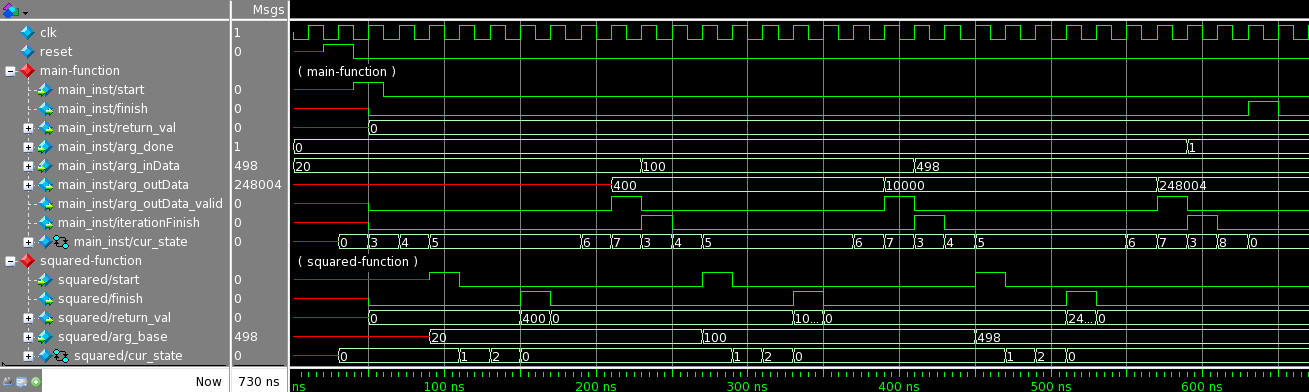
\includegraphics[width=0.99\textwidth]{../figs/SimulationWaveEX.png}
\caption{\label{fig:simulationwave}Simulation waveform of example design}
\end{figure}
\section{Synthesis}
The design is synthesized using a 180nm library. After synthesis, the circuitry of the design can be viewed in a GUI tool, but the output from LegUp is usually too large to understand. In \cref{fig:synthesiscircuittop} the top-module view from the tool is shown. The area and frequency reports from the synthesis is presented in \cref{tab:synthreportex}.

\begin{figure}[hbpt]
\centering
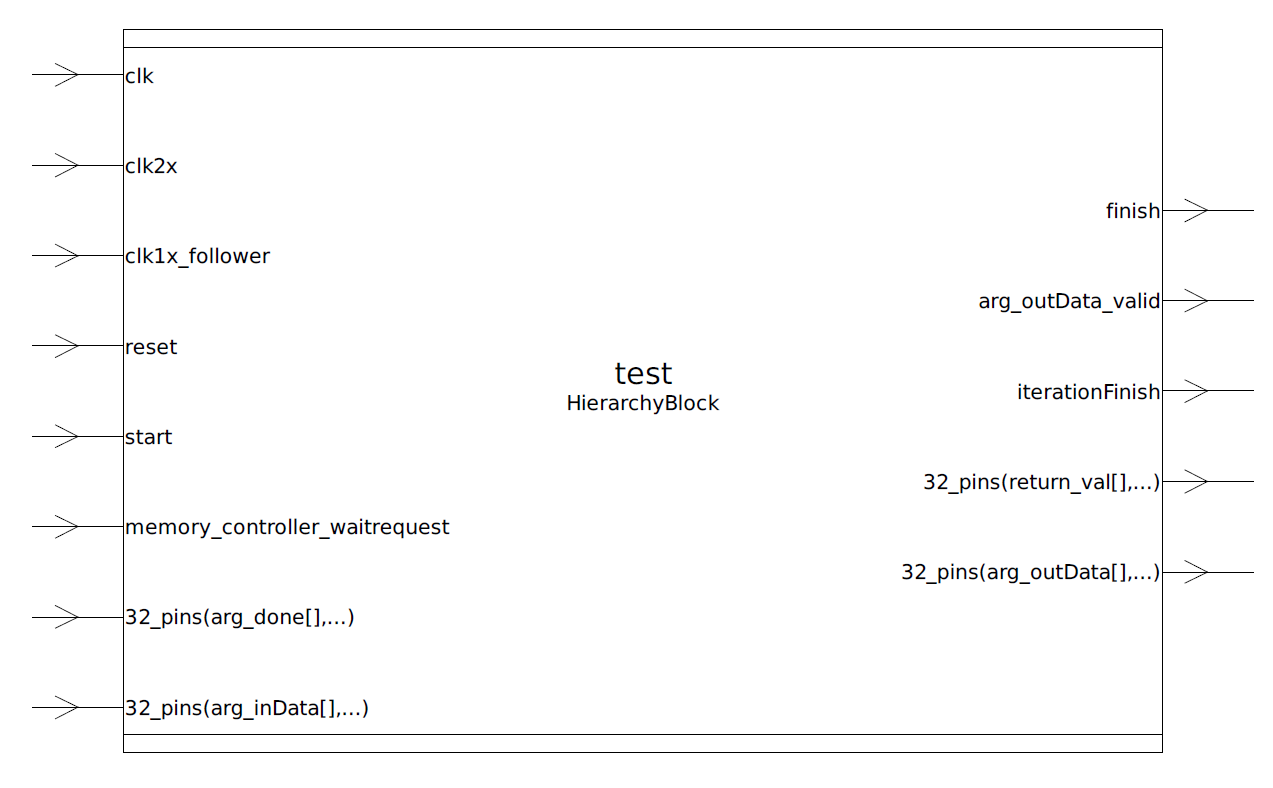
\includegraphics[width=0.99\textwidth]{../figs/SynthesisCircuit.png}
\caption{\label{fig:synthesiscircuittop}Top-level module generated by synthesis}
\end{figure}
\begin{table}[hbpt]
    \centering
    \begin{tabular}{lcr}
        \textbf{Parameter} && \textbf{Value} \\
        Combinational Area && 23853.614678 \\
        Noncombinational Area && 21015.456253 \\
        Buf/Inv Area && 1766.318423 \\
        Total Buffer Area && 39.92 \\
        Total Inverter Area && 1726.40 \\
        Macro/Black Box area && 0.000000 \\
        Net Interconnect area && 42732.128702 \\
        \midrule
        Total cell area && 44869.070931 \\
        Total area && 87601.199633 \\
        \midrule
        Critical Path Length && 27.43 ns \\
        Maximum Frequency && 36.46 MHz\\
        \bottomrule
    \end{tabular}
    \caption{Tool-flow example synthesis results}
    \label{tab:synthreportex}
\end{table}
To put the area of the synthesized design in perspective, the library defines a two-port NAND gate to be 9.9792 area units. The number of NAND2-equivalent gates for the design is then 8757 gates. This is a large amount for such a simple design, but the area overhead percentage of the design will shrink with larger designs. The area reported by synthesis is just an estimate, as layout can add optimizations to the design.
\section{Layout}
Layout is performed using the netlist from synthesis. After layout, it is possible to view the layout of the chip in a GUI-tool. The image in \cref{fig:layoutcircuit} shows the actual layout of the chip. The vertical yellow lines is power distribution to the teal horizontal lines, each purple boxes is a library cell, and the teal squares along the edges, marked \textit{I} or \textit{O}, are input and output ports of the chip. 
\begin{figure}[hbpt]
\centering
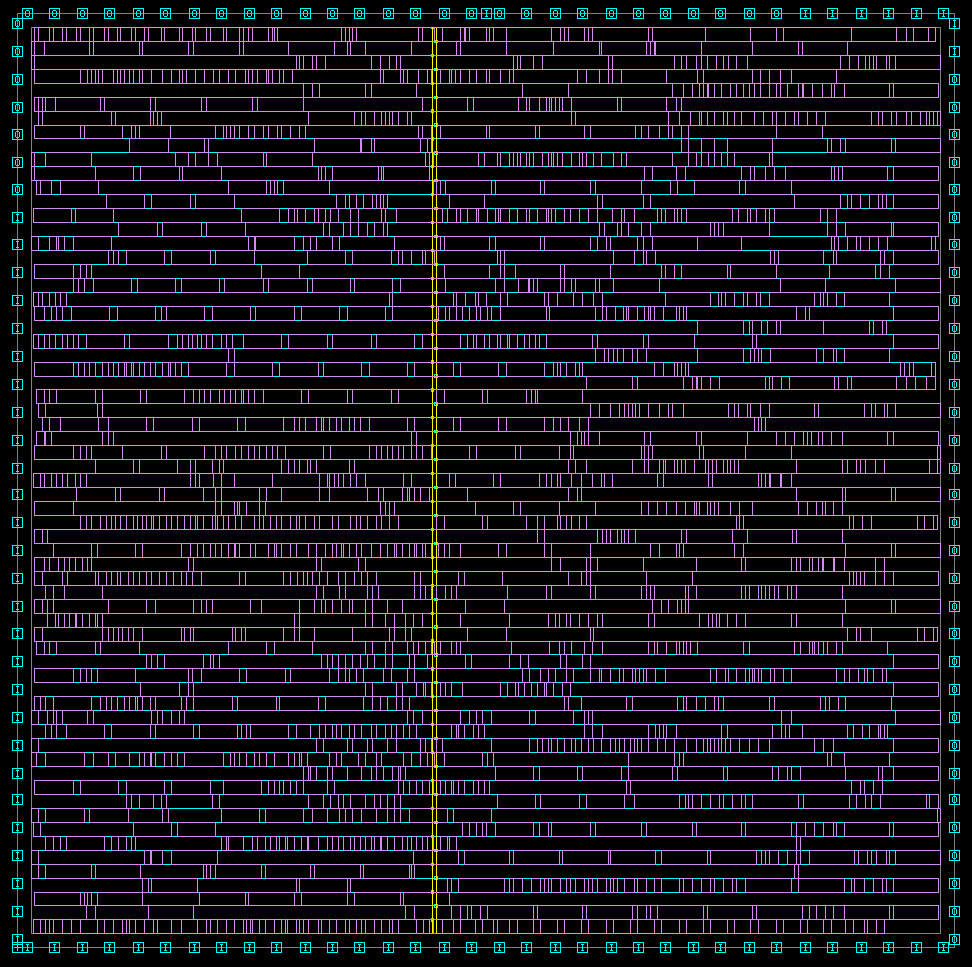
\includegraphics[width=0.99\textwidth]{../figs/LayoutCircuit.png}
\caption{\label{fig:layoutcircuit}Chip-layout of example design}
\end{figure}
Layout generates the final reports of area and critical path lengt. The reported values are listed in \cref{tab:layoutreportex}. Notice that the total area is reduced compared to the synthesis reports, while the critical path has increased a bit, leading to a decreased maximum frequency. The parameters \textit{Net XLength} and \textit{Net YLength} is the physical size of the chip, given in $\mu$m.

\begin{table}[hbpt]
    \centering
    \begin{tabular}{lcr}
        \textbf{Parameter} && \textbf{Value} \\
        \toprule
        Combinational Area && 24698.520289 \\
        Noncombinational Area && 18075.657349 \\
        Buf/Inv Area && 2577.960037 \\
        Total Buffer Area && 844.91 \\
        Total Inverter Area && 1733.05 \\
        Macro/Black Box Area && 0.000000 \\
        Net Area && 0.000000 \\
        Net XLength && 32867.52 \\
        Net YLength && 33528.53 \\
        \midrule
        Total cell area && 42774.177638 \\
        Total area && 42774.177638 \\
        Net Length && 66396.05 \\
        \midrule
        Critical Path Length && 28.51 ns \\
        Maximum Frequency && 35.08 MHz\\
        \bottomrule
    \end{tabular}
    \caption{Tool-flow example layout results}
    \label{tab:layoutreportex}
\end{table}

\section{Power estimation}
Power analysis uses switching data in the VCD- and SAIF-file generated under simulation to estimate the power consumption. As there are five different power scenarios defined, five results for each parameter is reported. The reporting from power analysis is shown in \cref{tab:powestreportex}. In this simple example, all power scenarios report the same power consumption, while in a larger design these values will vary. With a total estimated power consumption of 179.6$\mu$W, not much power is consumed in this chip, but again it is a small design.

\begin{table}[hbpt]
    \centering
    \begin{tabular}{lrccccc}
         & & \multicolumn{5}{c}{\textbf{Test \#}} \\
        \cline{3-7}
        \textbf{Parameter} &  & \textbf{crtl0} & \textbf{crtl1} & \textbf{crtl2} & \textbf{crtl3} & \textbf{inactive} \\
        \toprule
        Net Switching & [$\mu$W] & 27,33 & 27,33 & 27,33 & 27,33 & 27,33 \\
        Cell Internal & [$\mu$W] & 152,2 & 152,2 & 152,2 & 152,2 & 152,2 \\
        Cell Leakage & [nW] & 31,58 & 31,58 & 31,58 & 31,58 & 31,58 \\
        Total & [$\mu$W] & 179,6  & 179,6 & 179,6 & 179,6 & 179,6 \\
        \bottomrule
    \end{tabular}
    \caption{Tool-flow example power analysis results}
    \label{tab:powestreportex}
\end{table}